\chapter{智能合约运行时崩溃的预测方法探究}
\section{本章内容}
\label{sec:本章内容5}

智能合约在运行时可能因为发生异常而导致交易失败,然而,当前关于智能合约在运行时发生异常而崩溃的研究寥寥无几,因此本章在前文建立的数据集和漏洞检测模型的基础上,对智能合约运行时崩溃的预测方法进行了探索。本章首先对研究动机进行了阐述,然后对前文提出的静态代码指标进行了优化,并重新计算相关指标,最后针对新数据集进行标注并描述了标注的方法。最后一部分是在上一章的基础上开展了实验,融合专家特征和语义特征对预训练模型进行进一步训练,然后对实验结果进行了深入的分析。
\section{研究动机}
\label{sec:研究动机}
根据Siwapol等人的研究结果\cite{reducing2020},截止2020年,以太坊网络中由于执行交易失败的合约仅手续费已经消耗了超过2800万美元,消耗的区块奖励更是达到1210亿美元。针对这一现状,如果能在发送交易前,根据当前状态信息和即将调用的智能合约源代码对交易结果进行预测,提前发现可能失败的交易,便能节省交易手续费,同时在一定程度提高以太坊的运行效率。

智能合约在运行时可能因为发生异常而导致交易失败,以太坊官方文档中表明了失败交易的执行状态包括:Gas不足、Reverted、无效操作码、无效跳转和堆栈溢出。当然这只是对于交易失败状态的简单表述,具体的合约发生异常的原因多种多样,但是值得注意的是,智能合约被部署到以太坊网络上后,其字节码便不可再更改,也即合约每次被调用后的执行逻辑是完全相同的。因此本文认为,除了合约被调用时的输入和一些简单的状态信息外,合约执行失败的原因与其源代码本身有很大的关系,而上文的智能合约漏洞检测工作中,实验结果证明了静态代码指标和语义特征能充分表达智能合约源代码的结构特征和语义信息。鉴于此,本文尝试利用静态代码指标和语义特征对智能合约运行时是否会导致交易失败进行探索。


\section{实验数据集}
\label{sec:实验数据集}


% \textcolor{red}{这里可能要补充一些运行时的信息作为特征,不然可能会被喷:为什么同样的特征既可以用来检测漏洞也可以用来检测运行时异常?}
\subsection{静态代码指标优化}
在数据集方面,尽管\autoref{sec:基于静态度量定义专家特征}提出的34个静态代码指标能有效的表达程序的结构特征,但是对于智能合约运行时崩溃预测任务来说,有些指标对于合约执行逻辑的表达能力有限,因此本节对Solidity维度的静态代码指标进行了补充,并且删去一些相关性不大的指标,最终得到了25个静态代码指标,具体如\autoref{tab:new_metrics}所示。
\begin{table}[htbp]
    \caption{\label{tab:new_metrics}优化后的25个静态代码指标}
    \small
            \renewcommand{\arraystretch}{1.5}
        \begin{tabularx}{\linewidth}{cp{3.5cm}<{\centering}X<{\raggedright}}
            \hline
            \textbf{维度}            & \textbf{指标}              & \textbf{描述} \\ \hline
            \multirow{6}{*}{代码复杂度指标(6个)} & AvgComplexity        & 所有函数的圈复杂度的平均值 \\
                                       & MaxComplexity        & 所有函数的圈复杂度的最大值 \\
                                       & SumComplexity        & 所有函数的圈复杂度的总和 \\
                                       & MaxInheritance   & 主合约继承树的最大深度 \\
                                       & MaxNesting           & 主合约中控制结构的最深级别 \\
                                       & CountContractCoupled  & 与主合约存在耦合关系的合约的数量 \\ \hline
            \multirow{5}{*}{面向对象维度(5个)} & CountContractBase    &  主合约直接继承的合约的数量 \\
                                       & CountDependence      & 主合约直接或间接依赖的合约总数 \\
                                       & CountTotalFunction   & 主合约中定义的函数的总数 \\
                                       & CountFunctionPublic  & 主合约中定义的公开函数的个数 \\
                                       & CountVariable        & 主合约中定义的变量的个数 \\ \hline
            \multirow{14}{*}{Solidity维度(14个)} & NOI                 & 主合约中使用的接口总数 \\
                                       & NOL                & 主合约中使用的库合约总数\\
                                       & NOSV                & 主合约中定义的存储变量总数 \\
                                       & NOMap              & 主合约中使用的映射类型总数 \\
                                       & NOPay               & 主合约中调用的可支付函数总数 \\
                                       & NOE                 & 主合约中定义的事件总数 \\
                                       & NOMod               &  主合约中定义的函数修改器总数 \\
                                       & NOT                 & 主合约的所有函数中执行的转账语句总数 \\
                                       & NOC                 & 主合约中消息调用总数 \\
                                       & NODC                & 主合约的所有函数中执行的委托调用总数 \\
                                       & SDFB                & 主合约是否重写了 fallback 函数 \\ 
                                       & NOReq         & 主合约中require语句的个数 \\
                                       & NOAst         & 主合约中assert语句的个数 \\
                                       & NORvt         & 主合约中revert语句的个数 \\ \hline
        \end{tabularx}
\end{table}
\subsection{数据集标注与分析}
接下来要根据智能合约在以太坊中的交易情况对数据集进行标注,即确定一个合约是否会在被调用时发生异常而导致交易失败,本文称这些合约为崩溃合约。不同智能合约产生的交易数量差异较大,有些热门合约可能产生了成千上万笔交易,有些合约可能仅有3$\sim$5笔交易。Chen等人进行了一项研究\cite{chen2020understand}发现大约81\%的账户\footnote{96\%的智能合约账户和77\%的外部账户}在以太坊上的交易少于5次,也就是说大多数账户,尤其是智能合约账户并不频繁发起交易。此外,我们在BigQuery平台上对以太坊上智能合约及其交易信息进行了分析,结果表明94.3\%的合约的交易数在30以下(包含30)。因此,我们选择30次交易作为基准对原数据集进行过滤,删去交易次数大于30的智能合约,最终我们得到了一个包含\num{52638}份智能合约的数据集。
\begin{figure}[htbp]
    \centering
    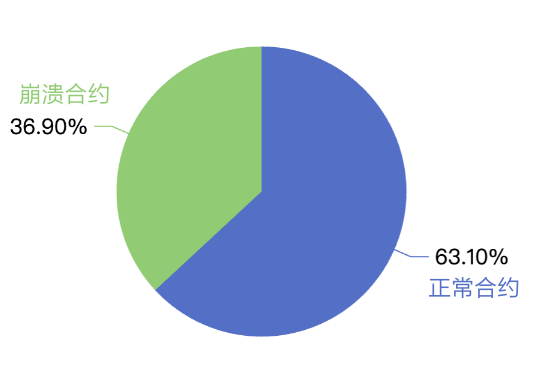
\includegraphics[width=.5\linewidth]{pictures/crash_no_crash2}
    \caption{\label{fig:crash_no_crash2}数据集中崩溃合约与正常合约的比例}
\end{figure}

下一步对数据集进行标注,如果一个智能合约的所有交易中只要产生了一次失败的交易,那么我们就标记这个合约为崩溃合约。以太坊中记录了智能合约的所有交易的执行结果,因此智能合约在运行时是否发生异常等信息都可以从以太坊网络获得,本文通过Etherscan提供的API来收集每一笔交易的执行结果,然后完成数据集的标注工作。数据集的统计信息如\autoref{fig:crash_no_crash2}所示。
从图中可以看出超过六成的智能合约都不是崩溃合约,仅有36.9\%的合约被标注为崩溃合约,这一现象合理解释是:大多数合约的交易总数较少,因此可能并未产生失败的交易。



% 最终,在54739份合约中,有xxx份被标记为崩溃合约,接下来我们将使用此数据集开展智能合约运行时崩溃预测的实验。



% 对数据集进行统计性分析
% 在数据集方面,我们沿用了从前文搜集的合约中提取出的专家特征和语义特征,但在标签上有一些不同。

% 智能合约在运行时可能发生的异常如xxx节所述,包括Gas不足、reverted、无效操作码、无效跳转和堆栈溢出。
% 下文将在运行时刻发生异常而崩溃的合约称为崩溃合约。

% 以太坊中记录了智能合约的所有交易的执行结果,因此智能合约在运行时是否发生异常等信息都可以从以太坊网络获得,本文通过Etherscan提供的API来收集每一笔交易的执行结果。

% 然而,不同的智能合约在以太坊中产生的交易数量差异较大,有些热门合约可能产生了成千上万笔交易(如0xab478a87c798789d80f800868667e),有些合约可能仅有3~5笔交易(如0xab478a87c798789d80f800868667e),本文对此情况的处理方法如下。

% 这里对各种运行时异常进行分析
\section{实验设计与结果分析}
\label{sec:实验设计与结果分析2}

\subsection{实验设计}
\label{sec:实验设计}
实验设计与上一章节的内容大致相同,即先使用编写好的程序为每一个智能合约计算新的静态代码指标,然后对其生成数据流图、控制流图和函数调用图,再利用GraphCodeBERT模型对源代码和语义图生成高维度的语义特征,最后融合基于静态代码指标的专家特征和语义特征,并使用线性分类器进行类别预测。每一步的细节都可以参考上一章节中的内容。另外,实验的运行环境、模型参数和结果评估指标等设置均遵循上一章节中的设定。
\subsection{实验结果分析}
\label{sec:实验结果分析2}
首先对交易执行失败的原因进行分析,从\autoref{fig:different_reasons}中可以看出,不同原因导致失败的交易在整个数据集中的分布并不均衡,其中占比最多的当属Reverted类型,紧接着是Gas不足,其次是无效操作码和无效跳转,堆栈溢出(上溢出或下溢出)占比非常之少,因此在相关的研究工作中可以忽略不计。对于其他四种导致交易失败的原因,本文且给出以下几点建议:
\begin{figure}[htbp]
    \centering
    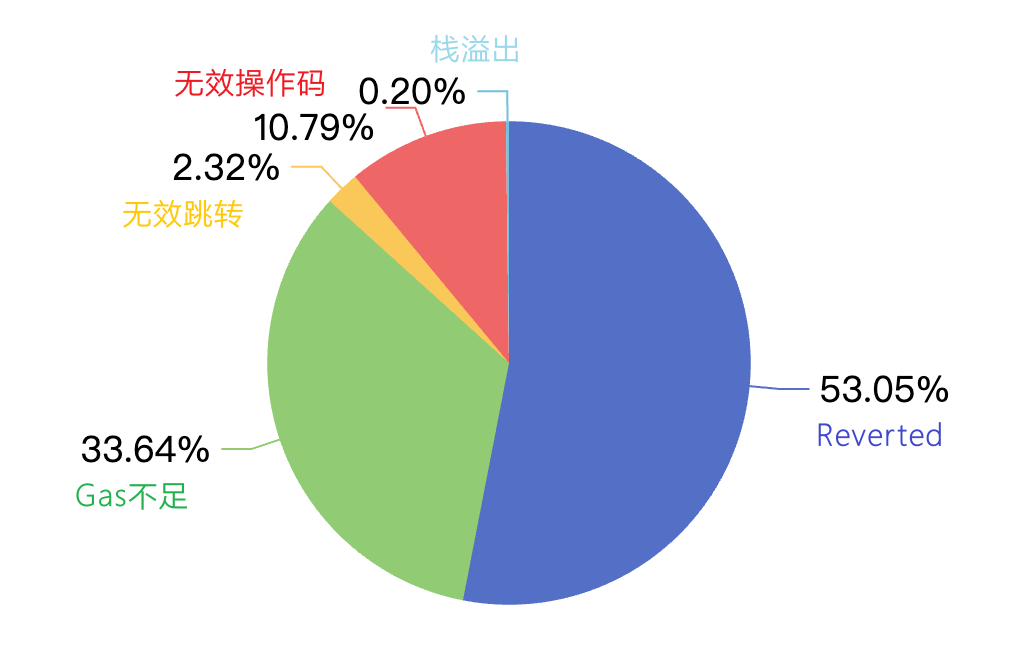
\includegraphics[width=.6\linewidth]{pictures/different_reasons}
    \caption{\label{fig:different_reasons}导致交易失败的不同原因在数据集中的分布情况}
\end{figure}

\begin{itemize}
    \item \textbf{Gas不足}。Gas不足的原因主要是发送交易前设置的Gas太少,或者智能合约编写不当。若 Gas 设置得过低,会导致交易失败,且发送交易前支付的矿工费依然会被收取。因此在设置 Gas 时,请设置得高一些以免交易失败,或者可以参照EIP-1559提案\cite{EIP1559}设置合适的gasPrice和gasLimit,其次检查智能合约源代码,避免出现死循环或过多耗时操作。
    \item \textbf{Reverted}。当智能合约运行结果为Reverted时,仅会扣除从合约执行开始到结束所消耗的Gas,所以如果不可避免地要使用require、assert或revert等函数时,请尽量减少他们的使用次数,并且提前它们在合约中的位置以减少可能的Gas消耗。
    \item \textbf{无效操作码}。这个错误通常和Solidity以及EVM的版本有关,在发布合约前最好对照官方文档使用匹配的Solidity编译器,及在源代码中正确地声明版本。
    \item \textbf{无效跳转}。这个错误通常是在调用合约时提供了无效的地址。比如一个合约调用了另一个合约的公开函数,被调用的合约地址作为调用参数被传入,如果传入的地址是虚构的,那么在合约执行时无法在区块链上找到对应的合约账户,因此就会导致该类异常。针对这个问题,建议在调用前使用assert或require等函数对参数进行检查。
\end{itemize}


\begin{figure}[htbp]
    \centering
    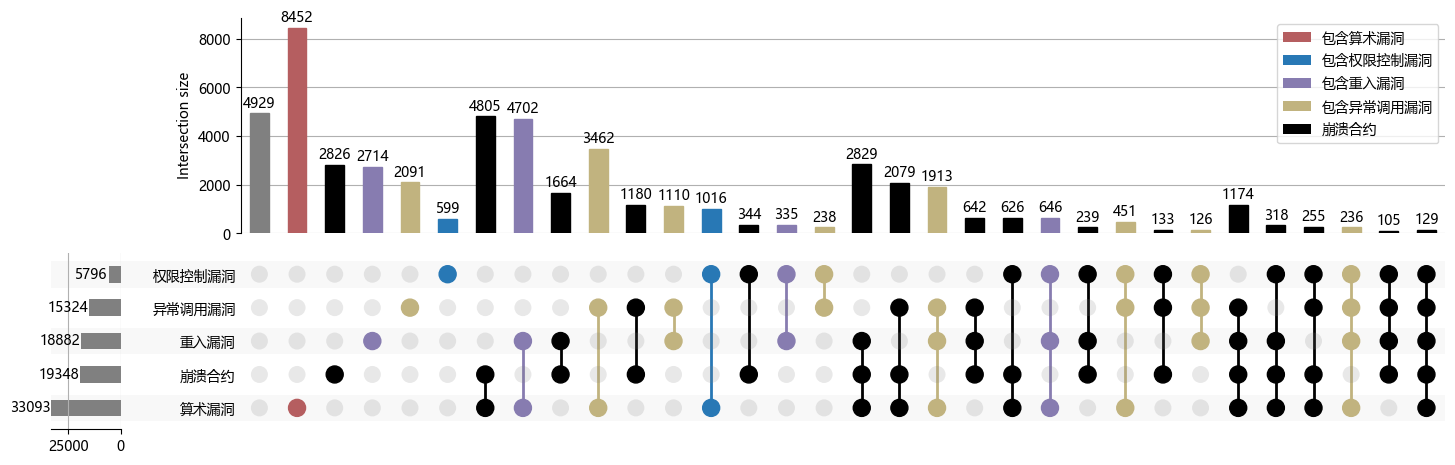
\includegraphics[width=\linewidth]{pictures/runtime_error_result}
    \caption{\label{fig:runtime_error_result}智能合约的四种漏洞与运行时崩溃的关系}
\end{figure}
使用上文得到的漏洞检测模型对优化后的数据集进行训练预测,三个指标Precision、Recall、F1-score的计算结果分别为0.83、0.76、0.79。这表明基于特征融合的预训练模型可以学习到智能合约的语义信息,可以在一定程度上对智能合约在运行时是否发生异常做出预测。

另一方面,本文进一步探究了上一章引入的智能合约的四种漏洞与合约因运行时异常而崩溃的关系,具体结果如\autoref{fig:runtime_error_result}所示。从图中可以看出,算术漏洞与合约崩溃的关系非常紧密,这可以解释为当除数为0时EVM会直接抛出异常并中止合约的执行;或者给变量的赋值超出了其存储范围从而导致其他计算结果的错误,最终合约无法结束导致Gas耗尽,最终崩溃。


% 基于特征融合的智能合约漏洞检测和运行时崩溃检测研究

% 漏洞检测预崩溃预测的关联

% 崩溃预测是最后一道防线,编写bug-free的程序才是最应该被重点关注的事,针对实验结果,提出以下几点针对性措施:

% 应对Gas不足的运行时异常,首先保证程序没有死循环

% revert操作码,尽量减少会导致revert的操作

% 无效操作码和无效跳转,尽量减少

% 若 Gas 设置得过低,会导致交易失败,且你所支付的矿工费依然会被以太坊网络收取,不会退回至你的钱包。因此在设置 Gas 时,请设置得高一些以免交易失败损失矿工费。

% 较低的矿工费可能会使交易确认时间延长,由于部分去中心化应用对交易时间有限制,过长的等待时间可能导致交易失败。

% 使用经济挡可能导致交易上链延迟。交易被打包上链的时间主要由两个因素决定:矿工费高低和网络拥堵程度。当网络拥堵时,交易可能需要更长的时间才能被矿工打包进区块。如果设置的矿工费过低,矿工可能会优先选择矿工费更高的交易,导致交易等待时间过长。
% \subsection{针对失败交易的建议}
% 不同原因导致失败的交易在整个数据集中的分布并不均衡,具体如\autoref{fig:runtime_error2}所示。可以看出,占比最多的当属revert类型,紧接着是Gas不足,其次是无效操作码和无效跳转,堆栈溢出(上溢出或下溢出)占比非常之少,因此在相关的研究工作中可以忽略不计。对于其他四种导致交易失败的原因,本文且给出以下几点建议:

% 不同原因导致失败的交易在整个数据集中的分布并不均衡,具体如\autoref{fig:runtime_error2}所示。可以看出,占比最多的当属revert类型,紧接着是Gas不足,其次是无效操作码和无效跳转,堆栈溢出(上溢出或下溢出)占比非常之少,因此在相关的研究工作中可以忽略不计。对于其他四种导致交易失败的原因,本文且给出以下几点建议:
% \begin{itemize}
%     \item \textbf{Gas不足}。Gas不足的原因主要是发送交易前设置的Gas太少,或者智能合约编写不当。若 Gas 设置得过低,会导致交易失败,且发送交易前支付的矿工费依然会被收取。因此在设置 Gas 时,请设置得高一些以免交易失败,或者可以参照EIP-1559提案\cite{EIP1559}设置合适的gasPrice和gasLimit,其次检查智能合约源代码,避免出现死循环或过多耗时操作。
%     \item \textbf{Reverted}。当智能合约运行结果为Reverted时,仅会扣除从合约执行开始到结束所消耗的Gas,所以如果不可避免地要使用require、assert或revert等函数时,请尽量减少他们的使用次数,并且提前它们在合约中的位置以减少可能的Gas消耗。
%     \item \textbf{无效操作码}。这个错误通常和Solidity以及EVM的版本有关,在发布合约前最好对照官方文档使用匹配的Solidity编译器,及在源代码中正确地声明版本。
%     \item \textbf{无效跳转}。这个错误通常是在调用合约时提供了无效的地址。比如一个合约调用了另一个合约的公开函数,被调用的合约地址作为调用参数被传入,如果传入的地址是虚构的,那么在合约执行时无法在区块链上找到对应的合约账户,因此就会导致该类异常。针对这个问题,建议在调用前使用assert或require等函数对参数进行检查。
% \end{itemize}
